% =========================================================
% CHAPITRE 3 — RÉALISATION
% =========================================================

\section{Introduction}

Après avoir présenté les besoins du système et défini son architecture
dans le chapitre précédent, cette partie est consacrée à la réalisation
du projet \textit{3awedlou}.

Cette étape présente les différents outils logiciels et matériels utilisés
pour développer et intégrer la solution. Elle décrit également le
processus global de fonctionnement du système, l'interface utilisateur
ainsi que le schéma de câblage de la partie électronique.

La réalisation a nécessité l'intégration de plusieurs domaines
technologiques, notamment les systèmes embarqués, l'électronique, la
communication IoT, le développement backend ainsi que le développement
d'interfaces web et mobiles.

\section{Outils et logiciels utilisés}

La réalisation du système \textit{3awedlou} s'appuie sur plusieurs outils
et environnements de développement. Chaque outil a été choisi en fonction
de son rôle dans l'une des différentes parties du projet.

\subsection{Arduino IDE}

Arduino IDE a été utilisé pour développer et téléverser les programmes
destinés aux microcontrôleurs utilisés dans la machine.

Il permet notamment de programmer l'Arduino Mega chargé d'assurer le
contrôle local de certains éléments de la machine, tels que le moteur
d'extrusion et le système de chauffage.

\begin{figure}[H]
    \centering
    
\includegraphics[width=0.14\textwidth]{figures/arduino-ide.png}
    \caption{Environnement Arduino IDE}
\end{figure}

\subsection{Visual Studio Code}

Visual Studio Code a été utilisé comme environnement principal pour le
développement des différentes parties logicielles du projet.

Il permet notamment de travailler sur le backend Symfony ainsi que sur les
applications web et mobiles.

\begin{figure}[H]
    \centering
    
\includegraphics[width=0.14\textwidth]{figures/vs-code.png}
    \caption{Environnement Visual Studio Code}
\end{figure}

\subsection{Symfony}

Symfony a été utilisé pour développer le backend de l'application. Il
assure notamment la gestion des utilisateurs, des machines, des sessions,
des données de télémétrie et des informations relatives à la production.

Le backend constitue également une couche intermédiaire entre
l'infrastructure IoT et les applications clientes.

\begin{figure}[H]
    \centering
    
\includegraphics[width=0.14\textwidth]{figures/symfony.png}
    \caption{Framework Symfony}
\end{figure}

\subsection{React}

React a été utilisé pour développer l'interface web de supervision. Il
permet de construire une interface composée de composants réutilisables
et d'afficher dynamiquement les informations provenant du backend.

\begin{figure}[H]
    \centering
    
\includegraphics[width=0.14\textwidth]{figures/react.png}
    \caption{Bibliothèque React}
\end{figure}

\subsection{React Native et Expo}

React Native a été utilisé pour développer l'application mobile
permettant d'accéder aux fonctionnalités du système depuis un
smartphone.

L'environnement Expo a facilité le développement, les tests et
l'exécution de l'application sur un appareil mobile.

\begin{figure}[H]
    \centering
    
\includegraphics[width=0.22\textwidth]{figures/react-native-expo.png}
    \caption{React Native et Expo}
\end{figure}

\subsection{PostgreSQL}

PostgreSQL a été utilisé comme système de gestion de base de données. Il
permet de stocker les informations relatives aux utilisateurs, aux
machines, aux sessions de fonctionnement, aux données de télémétrie et
aux productions.

\begin{figure}[H]
    \centering
    
\includegraphics[width=0.14\textwidth]{figures/postgresql.png}
    \caption{Système de gestion de base de données PostgreSQL}
\end{figure}

\subsection{Docker}

Docker a été utilisé pour faciliter l'exécution et la gestion de certains
services nécessaires au fonctionnement du backend, notamment la base de
données PostgreSQL.

Cette approche permet d'obtenir un environnement de développement plus
reproductible et plus facile à configurer.

\begin{figure}[H]
    \centering
    
\includegraphics[width=0.14\textwidth]{figures/docker.png}
    \caption{Outil de conteneurisation Docker}
\end{figure}

\subsection{Git et GitHub}

Git a été utilisé pour assurer le suivi des versions du code source.
GitHub permet de centraliser le dépôt du projet et de faciliter la
sauvegarde ainsi que la gestion des différentes versions du système.

\begin{figure}[H]
    \centering
    
\includegraphics[width=0.14\textwidth]{figures/git-github.png}
    \caption{Outils de gestion de versions Git et GitHub}
\end{figure}

\subsection{Outils de conception}
Des outils de conception assistée par ordinateur ont également été
utilisés pour concevoir et modifier les différents éléments mécaniques de
la machine.

La conception des pièces et de la structure mécanique permet d'adapter
les différents composants afin de répondre aux contraintes du système.

\subsubsection{SolidWorks}
SolidWorks a été utilisé pour concevoir les pièces mécaniques de la machine. Il permet de créer des modèles 3D précis et de simuler le
fonctionnement des mécanismes avant leur fabrication.

\begin{figure}[H]
    \centering
    
\includegraphics[width=0.14\textwidth]{figures/solid-works.png}
    \caption{Logiciel de conception mécanique SolidWorks}
\end{figure}

\subsubsection{Fritzing}
Fritzing a été utilisé pour concevoir les schémas électroniques et le câblage de la machine. Il permet de représenter visuellement les
connexions entre les différents composants électroniques et de faciliter la compréhension du circuit.

\begin{figure}[H]
    \centering
    
\includegraphics[width=0.14\textwidth]{figures/fritzing.png}
    \caption{Logiciel de conception électronique Fritzing}
\end{figure}


\section{Matériel utilisé}

La réalisation de la machine nécessite plusieurs composants électroniques,
mécaniques et électromécaniques.

\subsection{Arduino Mega}

L'Arduino Mega constitue l'un des principaux contrôleurs de la machine.
Il est chargé d'assurer le contrôle local de plusieurs fonctions,
notamment la commande du moteur pas à pas et la gestion du système de
chauffage.

Son nombre important d'entrées et de sorties permet également d'intégrer
plusieurs capteurs et actionneurs dans le même système.

\begin{figure}[H]
    \centering
    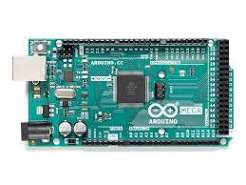
\includegraphics[width=0.2\textwidth]{figures/arduino-mega.png}
    \caption{Carte microcontrôleur Arduino Mega}
\end{figure}

\subsection{ESP32 DEVKIT V1}

Un ESP32 est intégré au système afin d'assurer les fonctions de
communication réseau et l'intégration de la machine dans l'architecture
IoT.

L'ESP32 permet notamment d'établir la communication avec le réseau et de
participer aux échanges de données avec l'infrastructure MQTT.

\begin{figure}[H]
    \centering
    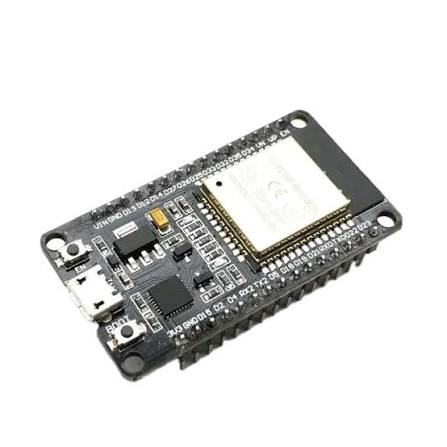
\includegraphics[width=0.18\textwidth]{figures/esp32.png}
    \caption{Carte de développement ESP32 DEVKIT V1}
\end{figure}

\subsection{Moteur pas à pas}

Un moteur pas à pas de type 42BYGH48-23D est utilisé pour assurer
l'entraînement du mécanisme d'extrusion.

Le moteur permet de contrôler précisément le déplacement du mécanisme
grâce à la commande de ses pas.

\begin{figure}[H]
    \centering
    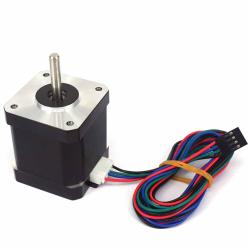
\includegraphics[width=0.2\textwidth]{figures/42bygh48-23d-moteur-pas-a-pas.png}
    \caption{Moteur pas à pas 42BYGH48-23D}
\end{figure}

\subsection{Module moteur pas à pas A4988}

Le moteur pas à pas est commandé à l'aide d'un driver A4988. Celui-ci
permet d'adapter les signaux de commande provenant du microcontrôleur afin
de piloter correctement le moteur.

Le driver permet également d'utiliser différents modes de micro-pas afin
d'améliorer la précision du mouvement.

\begin{figure}[H]
    \centering
    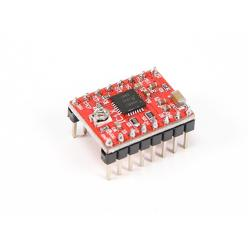
\includegraphics[width=0.2\textwidth]{figures/A4988-driver.png}
    \caption{Driver moteur pas à pas A4988}
\end{figure}

\subsection{Système de chauffage}

Un élément chauffant est utilisé pour chauffer le matériau PET jusqu'à
une température permettant sa transformation et son extrusion.

La température est mesurée à l'aide d'une thermistance et contrôlée par
le système embarqué afin de maintenir une température adaptée au
processus.

\begin{figure}[H]
    \centering
    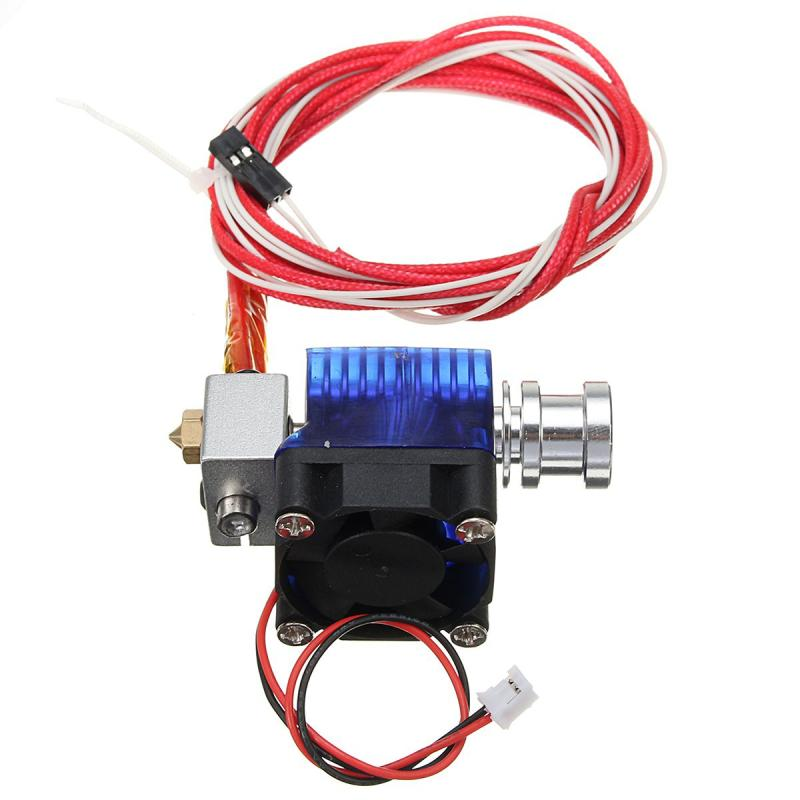
\includegraphics[width=0.23\textwidth]{figures/extrudeuse-simple-tete-17503mm-pour-imprimante-3d-12v.png}
    \caption{Tête d'extrusion chauffante}
\end{figure}

\subsection{Capteur de température}

Une thermistance est utilisée pour mesurer la température du système de
chauffage.

La valeur mesurée est récupérée par le microcontrôleur puis utilisée dans
la boucle de contrôle de température.

\subsection{Module de puissance BTS7960}

Un module de puissance est utilisé pour commander l'élément chauffant à
partir du microcontrôleur.

Cette interface permet de séparer la partie de commande basse tension de
la partie de puissance nécessaire au chauffage.

\begin{figure}[H]
    \centering
    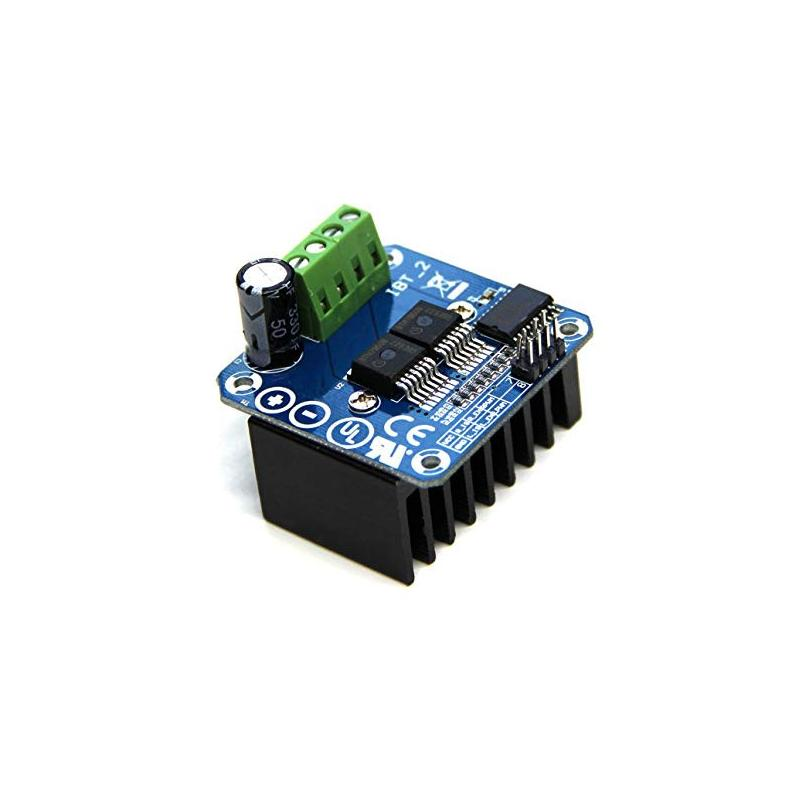
\includegraphics[width=0.2\textwidth]{figures/bts7960.png}
    \caption{Module de puissance BTS7960}
\end{figure}

\subsection{Convertisseur de niveau logique TXS0108}

Un convertisseur de niveau logique est utilisé pour assurer
l'adaptation des niveaux de tension entre les composants fonctionnant sous
différentes tensions logiques.

Cette adaptation est particulièrement importante pour la communication
entre l'Arduino Mega et l'ESP32.

\begin{figure}[H]
    \centering
    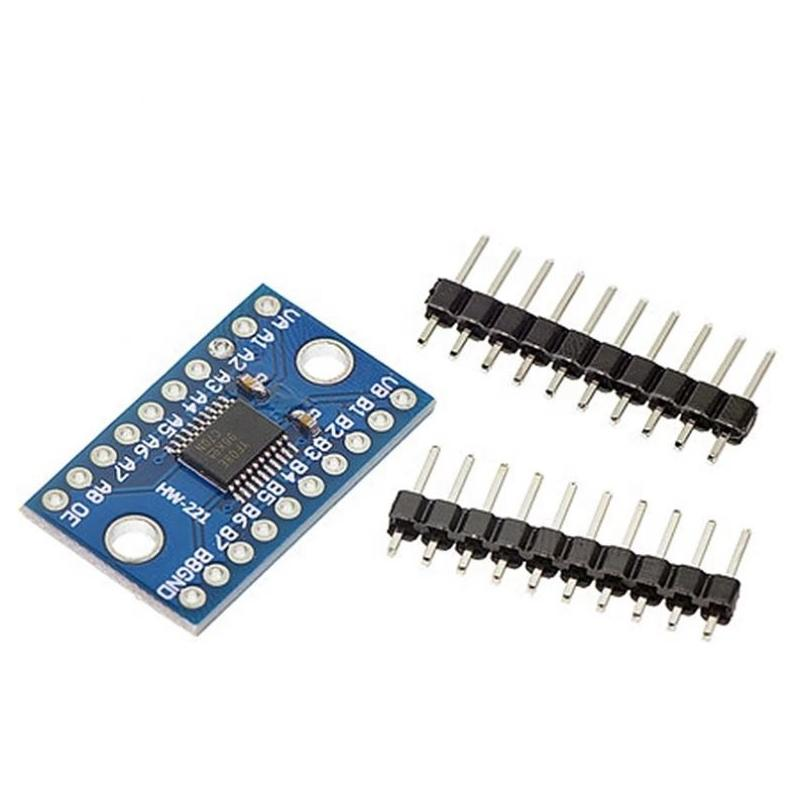
\includegraphics[width=0.2\textwidth]{figures/TXS0108E.png}
    \caption{Convertisseur de niveau logique TXS0108E}
\end{figure}

\subsection{Module convertisseur XL6009E1}
Deux modules convertisseur DC-DC sont utilisés pour fournir les tensions
nécessaires aux microcontrôleurs du système (9v pour l'Arduino Mega et 5v pour l'ESP32).

\begin{figure}[H]
    \centering
    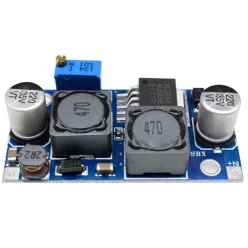
\includegraphics[width=0.2\textwidth]{figures/module-convertisseur-xl6009e.png}
    \caption{Module convertisseur DC-DC XL6009E1}
\end{figure}

\subsection{Alimentation}

La machine utilise une alimentation électrique adaptée aux différents
éléments du système.

Les tensions nécessaires aux composants sont obtenues directement ou à
l'aide de convertisseurs DC-DC afin de fournir des niveaux de tension
appropriés aux circuits électroniques.

\section{Processus du système}

Le fonctionnement général du système peut être décomposé en plusieurs
étapes successives.

\subsection{Préparation du matériau}

Le processus commence par la récupération et la préparation du plastique
PET destiné au recyclage. Le matériau doit être préparé avant son
introduction dans la machine afin de permettre son traitement dans de
bonnes conditions.

\subsection{Mise en température}

Après le démarrage de la machine, le système active le chauffage et mesure
continuellement la température à l'aide de la thermistance.

Le contrôleur compare la température mesurée avec la température de
consigne afin de maintenir les conditions nécessaires à l'extrusion.

\subsection{Extrusion}

Lorsque la température nécessaire est atteinte, le système peut démarrer
le mécanisme d'extrusion.

Le moteur pas à pas entraîne le mécanisme permettant de déplacer le
matériau à travers la zone chauffée. Le PET est ainsi transformé puis
extrudé sous forme de filament.

\subsection{Transmission des données}

Pendant le fonctionnement de la machine, les informations importantes
sont collectées par le système embarqué.

L'Arduino Mega communique avec l'ESP32, qui assure ensuite la transmission
des données vers l'infrastructure IoT.

Les informations peuvent notamment concerner l'état de la machine, la
température et les paramètres associés au processus de production.

\subsection{Supervision}

Les données transmises par la machine sont traitées par le backend puis
mises à disposition des applications web et mobile.

L'utilisateur peut ainsi consulter l'état de la machine et suivre les
informations relatives à son fonctionnement.

\subsection{Fin de production}

À la fin du processus, le système arrête progressivement les éléments
nécessaires au fonctionnement de la machine et enregistre les
informations relatives à la session de production.

Ces données peuvent ensuite être consultées à travers les interfaces de
supervision.

% Insérer ici un schéma du processus global.
%
% \begin{figure}[H]
%     \centering
%     \includegraphics[width=0.9\textwidth]{figures/system-process.png}
%     \caption{Processus global du système}
%     \label{fig:system-process}
% \end{figure}

\section{Interface utilisateur}

L'application \textit{3awedlou} comprend des interfaces permettant à
l'utilisateur de superviser le fonctionnement de la machine et de
consulter les informations disponibles.

Le système comprend une application web ainsi qu'une application mobile.
Les deux interfaces utilisent le même backend afin de centraliser la
gestion des données et des fonctionnalités.

\subsection{Application web}

L'application web constitue une interface de supervision accessible
depuis un navigateur.

Elle permet notamment de consulter les machines disponibles, leur état
actuel ainsi que les informations relatives aux sessions et à la
production.

% Insérer ici les captures de l'application web.
%
% \begin{figure}[H]
%     \centering
%     \includegraphics[width=0.9\textwidth]{figures/web-dashboard.png}
%     \caption{Interface web de supervision}
%     \label{fig:web-dashboard}
% \end{figure}

\subsection{Application mobile}

L'application mobile permet d'accéder aux fonctionnalités principales du
système depuis un smartphone.

Elle reprend les principales fonctions de supervision tout en adaptant
l'organisation des informations à la taille et aux contraintes d'un
écran mobile.

% Insérer ici les captures de l'application mobile.
%
% \begin{figure}[H]
%     \centering
%     \includegraphics[width=0.45\textwidth]{figures/mobile-dashboard.png}
%     \caption{Interface mobile de supervision}
%     \label{fig:mobile-dashboard}
% \end{figure}

\subsection{Communication avec le backend}

Les applications web et mobile communiquent avec le backend afin
d'accéder aux données et aux fonctionnalités du système.

Le backend centralise notamment l'authentification, la gestion des
machines, les données de télémétrie et les informations relatives aux
productions.

Cette architecture permet aux différentes interfaces d'utiliser une
source de données commune tout en conservant une séparation entre la
présentation et la logique métier.

\section{Schéma et câblage}

La réalisation matérielle nécessite l'interconnexion de plusieurs
composants électroniques. Le câblage a été conçu afin de séparer les
différentes fonctions de commande, de puissance, de mesure et de
communication.

L'Arduino Mega assure le contrôle de la partie locale de la machine. Il
est connecté au driver A4988 afin de commander le moteur pas à pas et au
circuit de puissance permettant de piloter le système de chauffage.

La thermistance est connectée à une entrée analogique afin de mesurer la
température du système. Les données de température sont ensuite utilisées
par l'algorithme de contrôle.

L'ESP32 est connecté à l'Arduino Mega afin d'échanger les informations
nécessaires à la communication avec le système IoT. Une adaptation des
niveaux logiques est utilisée pour assurer la compatibilité électrique
entre les deux microcontrôleurs.

L'alimentation électrique est distribuée vers les différents composants
en fonction de leurs tensions et courants nécessaires. Une attention
particulière est portée à la séparation entre les circuits de puissance
et les circuits logiques.

% Insérer ici le schéma électrique complet.
%
% \begin{figure}[H]
%     \centering
%     \includegraphics[width=\textwidth]{figures/schematic-diagram.png}
%     \caption{Schéma électrique du système}
%     \label{fig:schematic}
% \end{figure}

\subsection{Communication Arduino Mega -- ESP32}

La communication entre l'Arduino Mega et l'ESP32 est réalisée à l'aide
d'une liaison série UART.

Cette liaison permet à l'Arduino Mega de transmettre les informations
relatives à l'état de la machine à l'ESP32. Dans le sens inverse, l'ESP32
peut transmettre certaines commandes ou informations nécessaires au
contrôle du système.

La communication série repose sur les lignes TX, RX et GND. Étant donné
que l'Arduino Mega utilise une logique de 5 V alors que l'ESP32 fonctionne
avec une logique de 3,3 V, un convertisseur de niveau logique est utilisé
afin d'assurer une communication compatible avec les deux circuits.

% Insérer ici un schéma simplifié de la liaison UART.
%
% \begin{figure}[H]
%     \centering
%     \includegraphics[width=0.75\textwidth]{figures/uart-communication.png}
%     \caption{Communication UART entre l'Arduino Mega et l'ESP32}
%     \label{fig:uart}
% \end{figure}

\subsection{Commande du moteur}

Le moteur pas à pas est commandé par le driver A4988. L'Arduino Mega
génère les signaux nécessaires à son fonctionnement, notamment les
signaux \textit{STEP} et \textit{DIR}.

Le réglage du driver permet de définir le mode de micro-pas utilisé et
ainsi d'adapter la précision et la vitesse du mouvement aux besoins du
mécanisme d'extrusion.

\subsection{Contrôle de la température}

Le contrôle de la température constitue une fonction importante de la
machine. La thermistance fournit une mesure de la température au
microcontrôleur.

Cette mesure est ensuite utilisée par l'algorithme de régulation afin
d'ajuster la puissance appliquée au système de chauffage et de maintenir
la température autour de la valeur de consigne.

% Insérer ici un schéma du contrôle de température.
%
% \begin{figure}[H]
%     \centering
%     \includegraphics[width=0.85\textwidth]{figures/temperature-control.png}
%     \caption{Principe de contrôle de la température}
%     \label{fig:temperature-control}
% \end{figure}

\section{Conclusion}

Ce chapitre a présenté la réalisation du système \textit{3awedlou}, depuis
les outils de développement et les composants matériels jusqu'à
l'intégration des différents éléments de la solution.

La partie embarquée permet d'assurer le contrôle local de la machine,
tandis que l'ESP32 assure la connectivité nécessaire à son intégration
dans l'architecture IoT. Le backend centralise la gestion des données et
les applications web et mobile permettent leur consultation et leur
supervision.

La réalisation matérielle, le câblage et les différents mécanismes de
communication permettent ainsi de réunir les différentes composantes du
projet au sein d'un système cohérent.

Les résultats obtenus constituent une base permettant de poursuivre les
tests du système, d'améliorer sa fiabilité et d'optimiser le processus de
recyclage et de production du filament.